\documentclass[12pt,
border=1pt]{standalone}
\usepackage{pgfplots}
\usepackage{amsmath}
\usepackage{amssymb}

\pgfplotsset{compat=newest,
	width=6cm, height=5cm,
	xtick pos=left, ytick pos=left,
	%            scaled x ticks=real:1e-6,
}
% Kernel 2 FP64
\begin{document}
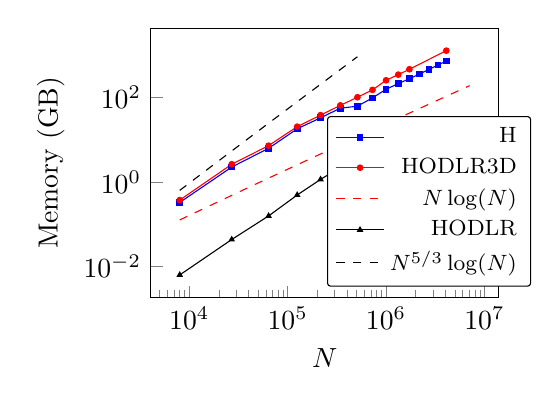
\begin{tikzpicture}[every mark/.append style={mark size=1pt}]
	\begin{axis}[xlabel={$N$},
	ylabel={Memory (GB)},
%		legend pos=south east,
		legend style={
                at={(0.8,0.04)},
               anchor=south,
               legend columns=1,
               cells={anchor=east},
              font=\footnotesize,
               rounded corners=1pt,
               },
		xmode = log,
	    ymode = log,
	   % xmin = 1e3,
	   % xmax = 1e6,
	   % ymin = 1e-10,
	   % ymax = 1e-0,
	   % xtick={1e-10, 1e-8, 1e-6,  1e-4,  1e-2},
	   % ytick={1e-8, 1e-6,  1e-4,  1e-2, 1e-0}
		]
		
		\addplot[
		color=blue,
		mark=square*,
		] coordinates {
(8000, 64* 0.005058)
(27000, 64* 0.035003)
(64000, 64* 0.097724)
(125000, 64* 0.283650)
(216000, 64* 0.518278)
(343000, 64* 0.876862)
(512000, 64* 0.979559)
(729000, 64* 1.543490)
(1000000, 64* 2.469610)
(1331000, 64* 3.369570)
(1728000, 64* 4.393640)
(2197000, 64* 5.723660)
(2744000, 64* 7.381680)
(3375000, 64* 9.338010)
(4096000, 64* 11.514600)
% (4913000, 64* 14.384300)
% (5832000, 64* 17.765400)
% (6859000, 64* 21.766000)
		};
		\addplot[
		color=red,
		mark=*,
		] coordinates {
(8000, 64* 0.005755)
(27000, 64* 0.040850)
(64000, 64* 0.113066)
(125000, 64* 0.319833)
(216000, 64* 0.599801)
(343000, 64* 1.023840)
(512000, 64* 1.597820)
(729000, 64* 2.389400)
(1000000, 64* 4.033750)
(1331000, 64* 5.495990)
(1728000, 64* 7.382610)
(4096000, 64* 20.424200)
		};
		\addplot[mark=none, red, dashed][
		domain = 8000:7077888,
		] {(pow(10,-5.4)*x*log10(x)};
\addplot[
		color=black,
		mark=triangle*,
		] coordinates {
(8000,0.006124)
(27000,0.042521)
(64000,0.154553)
(125000,0.485584)
(216000,1.139310)
(343000,2.225850)
(512000,4.058760)
		};
\addplot[mark=none, black, dashed][
		domain = 8000:512000,
		] {(pow(10,-7.3)*pow(x,5/3)*log10(x)};
		
		\legend{H, HODLR3D, $N\log(N)$, HODLR, $N^{5/3}\log(N)$}	
		\end{axis}
\end{tikzpicture}
\end{document}